\documentclass{beamer}\usepackage[]{graphicx}\usepackage[]{color}
% maxwidth is the original width if it is less than linewidth
% otherwise use linewidth (to make sure the graphics do not exceed the margin)
\makeatletter
\def\maxwidth{ %
  \ifdim\Gin@nat@width>\linewidth
    \linewidth
  \else
    \Gin@nat@width
  \fi
}
\makeatother

\definecolor{fgcolor}{rgb}{0.345, 0.345, 0.345}
\newcommand{\hlnum}[1]{\textcolor[rgb]{0.686,0.059,0.569}{#1}}%
\newcommand{\hlstr}[1]{\textcolor[rgb]{0.192,0.494,0.8}{#1}}%
\newcommand{\hlcom}[1]{\textcolor[rgb]{0.678,0.584,0.686}{\textit{#1}}}%
\newcommand{\hlopt}[1]{\textcolor[rgb]{0,0,0}{#1}}%
\newcommand{\hlstd}[1]{\textcolor[rgb]{0.345,0.345,0.345}{#1}}%
\newcommand{\hlkwa}[1]{\textcolor[rgb]{0.161,0.373,0.58}{\textbf{#1}}}%
\newcommand{\hlkwb}[1]{\textcolor[rgb]{0.69,0.353,0.396}{#1}}%
\newcommand{\hlkwc}[1]{\textcolor[rgb]{0.333,0.667,0.333}{#1}}%
\newcommand{\hlkwd}[1]{\textcolor[rgb]{0.737,0.353,0.396}{\textbf{#1}}}%
\let\hlipl\hlkwb

\usepackage{framed}
\makeatletter
\newenvironment{kframe}{%
 \def\at@end@of@kframe{}%
 \ifinner\ifhmode%
  \def\at@end@of@kframe{\end{minipage}}%
  \begin{minipage}{\columnwidth}%
 \fi\fi%
 \def\FrameCommand##1{\hskip\@totalleftmargin \hskip-\fboxsep
 \colorbox{shadecolor}{##1}\hskip-\fboxsep
     % There is no \\@totalrightmargin, so:
     \hskip-\linewidth \hskip-\@totalleftmargin \hskip\columnwidth}%
 \MakeFramed {\advance\hsize-\width
   \@totalleftmargin\z@ \linewidth\hsize
   \@setminipage}}%
 {\par\unskip\endMakeFramed%
 \at@end@of@kframe}
\makeatother

\definecolor{shadecolor}{rgb}{.97, .97, .97}
\definecolor{messagecolor}{rgb}{0, 0, 0}
\definecolor{warningcolor}{rgb}{1, 0, 1}
\definecolor{errorcolor}{rgb}{1, 0, 0}
\newenvironment{knitrout}{}{} % an empty environment to be redefined in TeX

\usepackage{alltt}
\usetheme{Madrid}

%%%%% Packages %%%%%
\usepackage{algorithm}
\usepackage{csquotes}
\usepackage[round]{natbib}
\bibliographystyle{agsm}
\usepackage{algorithmic}
\usepackage{pgfpages}
\usepackage{ragged2e}
\usepackage{etoolbox}
\usepackage{lipsum}
\usepackage{subfig}
\apptocmd{\frame}{}{\justifying}{} 
\usepackage{xcolor}
\usepackage{dsfont}
\usepackage{tikz}
\usepackage{amsmath}
\usepackage{graphicx}
\usepackage{subfig}
\usepackage{mathtools}
\usepackage{xcolor}
\usepackage{comment}
\usepackage{appendixnumberbeamer}
%%%%% New Commands %%%%
\newcommand{\btheta}{\boldsymbol{\theta}}
\newcommand{\x}{\mathbf{x}}
\newcommand{\SUN}{\textrm{SUN}}
\newcommand{\X}{\mathbf{X}}
\newcommand{\T}{\textrm{T}}
\newcommand{\A}{\mathcal{A}}
\newcommand{\I}{\mathds{1}}
\newcommand{\hist}{\mathbb{H}_{t-1}}
\newcommand\myeq{\stackrel{\mathclap{\normalfont\mbox{def}}}{=}}
\def\app#1#2{%
  \mathrel{%
    \setbox0=\hbox{$#1\sim$}%
    \setbox2=\hbox{%
      \rlap{\hbox{$#1\propto$}}%
      \lower1.1\ht0\box0%
    }%
    \raise0.25\ht2\box2%
  }%
}
\def\approxprop{\mathpalette\app\relax}
%\pgfpagesuselayout{1 on 1}[a4paper,border shrink=5mm]
\title[DDE and PCB effect on Premature delivery]{Assessing Effects of Exposures to DDE and PCBs on Premature Delivery via Ordinal Logistic Regression}
\author[Morsomme, Ou, Zito]{Raphael Morsomme \and Rihui Ou \and Alessandro Zito}
\institute[Stat 723]{Case Study 1 - Stat 723}
\date{\today}
\IfFileExists{upquote.sty}{\usepackage{upquote}}{}
\begin{document}

\begin{frame}
\titlepage
\end{frame}

\begin{frame}{Overview}
\tableofcontents
\end{frame}

%%%%%%%%%%%%%%%%%%%%%%%%%%%%%%%%%%%%%%%%%%%%%
%%%% Introduction                       
%%%%%%%%%%%%%%%%%%%%%%%%%%%%%%%%%%%%%%%%%%%%%
\section{Introduction}
\begin{frame}{Introduction}
\begin{itemize}
\item \textcolor{red}{\textbf{Framework}}: \\
\textit{Dichlorodiphenyldichloroethylene} (DDE) and \textit{Polychlorinated Biphenyls} (PCBs) 
are chemicals that persist in the envirnoment and get stored in fatty depositis in the human tissues.\\
$\quad \Longrightarrow \ $\textcolor{blue}{Potential adverse effect on health}
\item \textcolor{red}{\textbf{Question}}:\\
\textit{Is exposure to DDE and PBCs associated with a higher chance of premature delivery in pregnant women?}
\end{itemize}
\begin{block}{Pregnancy timeline}
\begin{itemize}
\item \textbf{Dangerous preterm}:  delivery at 34 weeks or before (when main organs are underdeveloped)
\item \textbf{Preterm}: delivery beween 35 and 37 week
\item \textbf{At term}: delivery after 37 weeks
\end{itemize}
\end{block}
\end{frame}

%%%%%%%%%%%%%%%%%%%%%%%%%%%%%%%%%%%%%%%%%%%%%
%%%% The Data                       
%%%%%%%%%%%%%%%%%%%%%%%%%%%%%%%%%%%%%%%%%%%%%
\section{Data}
\begin{frame}{Data}
Data collected by 12 centers contained gestational age (in weeks) of the mother, the DDE and PCBs concentration, socio-economic info and scores (race, occupation, education, income), amount of triglycerides and cholesterol in blood and smoking status. \\
\medskip 
\textcolor{red}{\textbf{Preprocessing}}:
\begin{itemize}
\item Drop obs. with gestational age $>$ 45 (the world record)
\item Standardize and average levels of PCBs\footnote{This avoids the correlation between the PCBs. See the appendix.}
$$PCB_i = \frac{1}{11}\sum_{j=1}^{11} \frac{PCB_{ij} - mean_i(PCB_{ij})}{sd_i(PCB_{ij})}$$
\item Mean impute of occupation, education and income scores 
\item Aggregate race into $race = 1$ if white and $race=0$ if non-white
\end{itemize}
$\quad \Longrightarrow$ \textcolor{blue}{Total obs.} = \textbf{2336}
\end{frame}
%%%%%%%%%%%%%%%%%%%%%%%%%%%%%%%%%%%%%%%%%%%%
\begin{frame}{Data}
\small
\begin{itemize}
\item \textbf{Our dependent varible is}:
$$gestgroup_i = 
\begin{cases}
0 & if \ \textrm{Dangerous preterm} \\
1 & if \ \textrm{Preterm} \\
2 & if \ \textrm{At term} 
\end{cases}$$
\item To account for triglyceredes and cholesterol, we introduce an \textbf{adjusted measure for} $PCB$ \textbf{and} $DDE$ by:
\begin{enumerate}
\item Computing total lipids using Phillips et al.(1989) and Bernert et al.(2007) forumula $$lipid_i =  2.27 * cholesterol_i + triglycerides_i + 0.623$$ 
\item Setting\footnote{The choice of the log comes from a Box-Cox analysis of the log-likelihood, as in Li, Longnecker and Dunson (2013)}
$$adjDDE_i = \frac{DDE_i}{log(lipid_i)} \qquad adjPCB_i = \frac{PCB_i}{log(lipid_i)}$$
\end{enumerate}
\end{itemize}
\end{frame}

%%%%%%%%%%%%%%%%%%%%%%%%%%%%%%%%%%%%%%%%%%%%%
%%%% EDA                    
%%%%%%%%%%%%%%%%%%%%%%%%%%%%%%%%%%%%%%%%%%%%%
\begin{frame}{EDA (I) - Exposures and gestational groups by race}

\begin{figure}
  \centering
  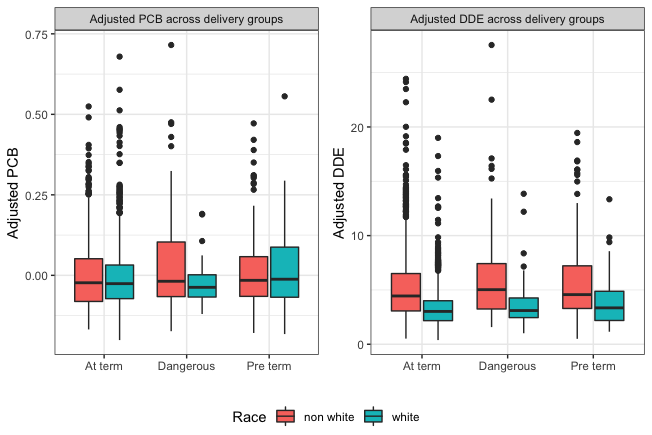
\includegraphics[width=0.8\textwidth]{Fig1-Adjusted_exposure_gestgroup.png}
\caption{Relationship between delivery group and adjusted exposures, by race}
\label{fig:p1}
\end{figure}
\end{frame}

\begin{frame}{EDA (II) - Exposure across centers}
% Ask Raphael to do this. Need a slide with distribution of DDE and PCB or gestgroup across centers
\end{frame}
%%%%%%%%%%%%%%%%%%%%%%%%%%%%%%%%%%%%%%%%%%%%%
%%%% Model 1                    
%%%%%%%%%%%%%%%%%%%%%%%%%%%%%%%%%%%%%%%%%%%%%
\section{Model (I) - Ordinal Logistic Regression}
% Insert here the AIC part
\begin{frame}{Model (I) - Ordinal Logistic Regression}
We run the following ordinal logistic regression model:
\begin{align*}
	\textrm{logit}(P(gestgroup \leq j)) = \beta_{0j} - \mathbf{X} \boldsymbol{\beta} + \boldsymbol{\varepsilon}
\end{align*}

where $j = 0,1,2$ corresponds to the outcome level, and \textbf{X} contains:
\begin{itemize}
	\item $adjDDE$, $adjPCB$, $race$, $center$, $smoke$, the 3 scores, and mother age [\textcolor{blue}{main effects}]
	\item ($adjDDE$ + $adjPCB$) * ($race$ + $center$) [\textcolor{blue}{interactions}].
\end{itemize}
\medskip
AIC-based backward variable selection:
\begin{itemize}
	\item \textcolor{blue}{Maintain} $DDE$, $PCB$, $smoke$, $center$, $race$, ($PCB$ + $DDE$) * $race$
	\item \textcolor{red}{Drop} ($DDE$ + $PCB$) * $center$ , mother age, 
\end{itemize}

Model assumptions are checked in the appendix.
\end{frame}


% https://www.ncbi.nlm.nih.gov/pmc/articles/PMC3812826/#R13
%%%%%%%%%%%%%%%%%%%%%%%%%%%%%%%%%%%%%%%%%%%%%
%%%% Model 2                   
%%%%%%%%%%%%%%%%%%%%%%%%%%%%%%%%%%%%%%%%%%%%%
\section{Model (II) - Bayesian Ordinal Logistic Regression}
\begin{frame}{Model (II) - Bayesian Ordinal Logistic Regression}
\end{frame}

%%%%%%%%%%%%%%%%%%%%%%%%%%%%%%%%%%%%%%%%%%%%%
%%%% Results
%%%%%%%%%%%%%%%%%%%%%%%%%%%%%%%%%%%%%%%%%%%%%
\section{Results}
\begin{frame}{Numerical Results}
\begin{tabular}{l|r|r}
\hline
  & 5\% & 95\%\\
\hline
dde\_env\_bc & -0.0513582 & 0.0097459\\
\hline
pcb\_env\_bc & -2.7673825 & -0.7043851\\
\hline
race\_aggwhite & 0.0854250 & 0.8561411\\
\hline
center10 & -0.1122673 & 0.7602643\\
\hline
center15 & -1.0956887 & -0.2863208\\
\hline
center31 & -0.2567563 & 0.8024497\\
\hline
center37 & -1.0273528 & -0.3027346\\
\hline
center45 & -0.4292124 & 0.3496075\\
\hline
center50 & -0.5401077 & 0.2402548\\
\hline
center55 & -0.7698277 & 0.0759588\\
\hline
center60 & -0.6561040 & 0.1663142\\
\hline
center66 & -0.4817386 & 0.1849701\\
\hline
center71 & -0.4542238 & 0.2900110\\
\hline
center82 & -1.0930024 & -0.2869819\\
\hline
smoking\_status1 & -0.3170003 & -0.0014069\\
\hline
dde\_env\_bc:race\_aggwhite & -0.1174506 & 0.0160157\\
\hline
pcb\_env\_bc:race\_aggwhite & -0.0290488 & 3.2124015\\
\hline
0Dangerous|1Pre term & -3.2503005 & -2.5306140\\
\hline
1Pre term|2At term & -1.8930640 & -1.2207209\\
\hline
\end{tabular}
\end{frame}
%%%%%%%%%%%%%%%%%%%%%%%%%%%%%%%%%%%%%%%%%%%%%
%%%% Results
%%%%%%%%%%%%%%%%%%%%%%%%%%%%%%%%%%%%%%%%%%%%%
\section{Results}
\begin{frame}{Graphical Results}

\end{frame}

%%%%%%%%%%%%%%%%%%%%%%%%%%%%%%%%%%%%%%%%%%%%%
%%%% Conclusions                  
%%%%%%%%%%%%%%%%%%%%%%%%%%%%%%%%%%%%%%%%%%%%%

\section{Conclusions}
\begin{frame}{Conclusions}
\end{frame}

%%%%%%%%%%%%%%%%%%%%%%%%%%%%%%%%%%%%%%%%%%%%%
%%%% Appendix                 
%%%%%%%%%%%%%%%%%%%%%%%%%%%%%%%%%%%%%%%%%%%%%
\appendix
\section{Appendix}
\begin{frame}{Appendix}{More EDA}
\begin{figure}
  \centering
  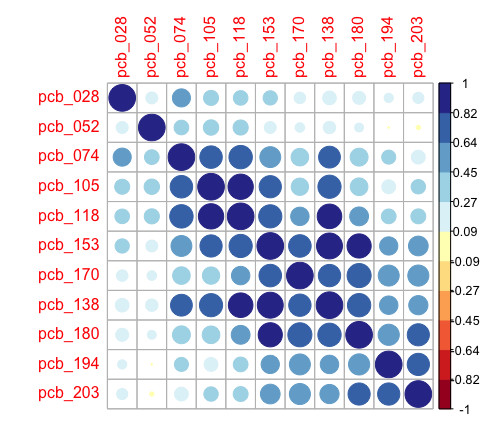
\includegraphics[width=0.6\textwidth]{corrplot_PCB.png}
\caption{Correlation plot across PCBs}
\label{fig:corrPCB}
\end{figure}
\end{frame}
%%%%%%%%%%%%%%%%%%%%%%%%%%%%%%%%%%%%%%%%%%%%%
\begin{frame}{Appendix}{Frequentist Model Checking}
We can check the assumption of the (frequentist) ordinal logistic model by looking at the Surrogate residuals. \textcolor{red}{ADD CITATION HERE}\\
\medskip
If the model assumptions are correct, then the surrogate residuals $R_S$ will have three properties:
\begin{enumerate}
 \item $E(R_S|X)=0$
 \item $Var(R_S|X)=c$, the conditional variance of $R_S$ is constant
 \item The emiprical distribution of $R_S$ resembles an explicit distribution that is related to the link function $G^{-1}(\cdot)$. Specifically, $R_S\sim G(c+\int ud G(u))$.
\end{enumerate}
\end{frame}
%%%%%%%%%%%%%%%%%%%%%%%%%%%%%%%%%%%%%%%%%%%%%
\begin{frame}{Appendix}{Frequentist Model Checking}

Assumptions (i) and (ii) are checked with the Surrogate residuals plot. Both are satisfied in this case.
\begin{figure}
  \centering
  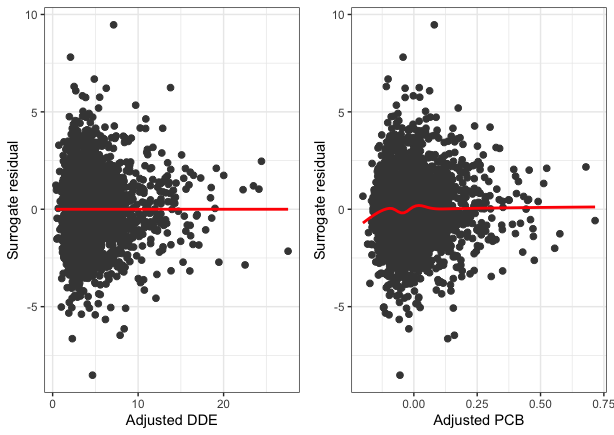
\includegraphics[width=0.7\textwidth]{Surrogate_residuals.png}
\caption{Surrogate residuals of DDE and PCB}
\label{fig:surrogateresid}
\end{figure}
\end{frame}
%%%%%%%%%%%%%%%%%%%%%%%%%%%%%%%%%%%%%%%%%%%%%
\begin{frame}{Appendix}{Frequentist Model Checking}

\begin{figure}
  \centering
  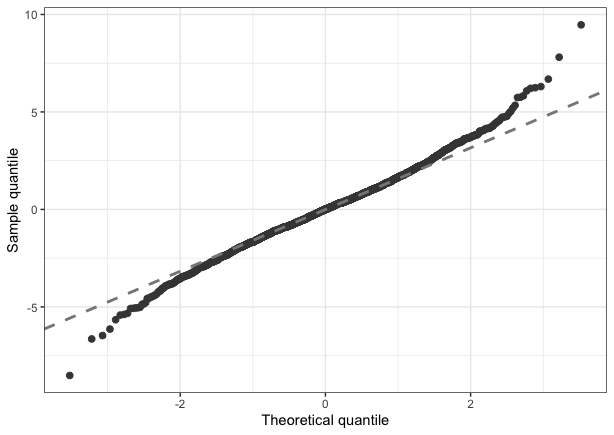
\includegraphics[width=0.7\textwidth]{qqplot.png}
\caption{QQ plot of the Surrogate residuals}
\label{fig:qqplot}
\end{figure}
\end{frame}
%%%%%%%%%%%%%%%%%%%%%%%%%%%%%%%%%%%%%%%%%%%%%
\begin{frame}{Appendix}{Box-Cox transformation of lipid}
Following Li, Longnecker and Dunson (2013), we adjust the exposures by dividing for a Box-Cox tranformation of the level of lipids. We see that the optimal $\lambda$ is at 0, which suggests a $\log$ transformation. 
\begin{knitrout}
\definecolor{shadecolor}{rgb}{0.969, 0.969, 0.969}\color{fgcolor}
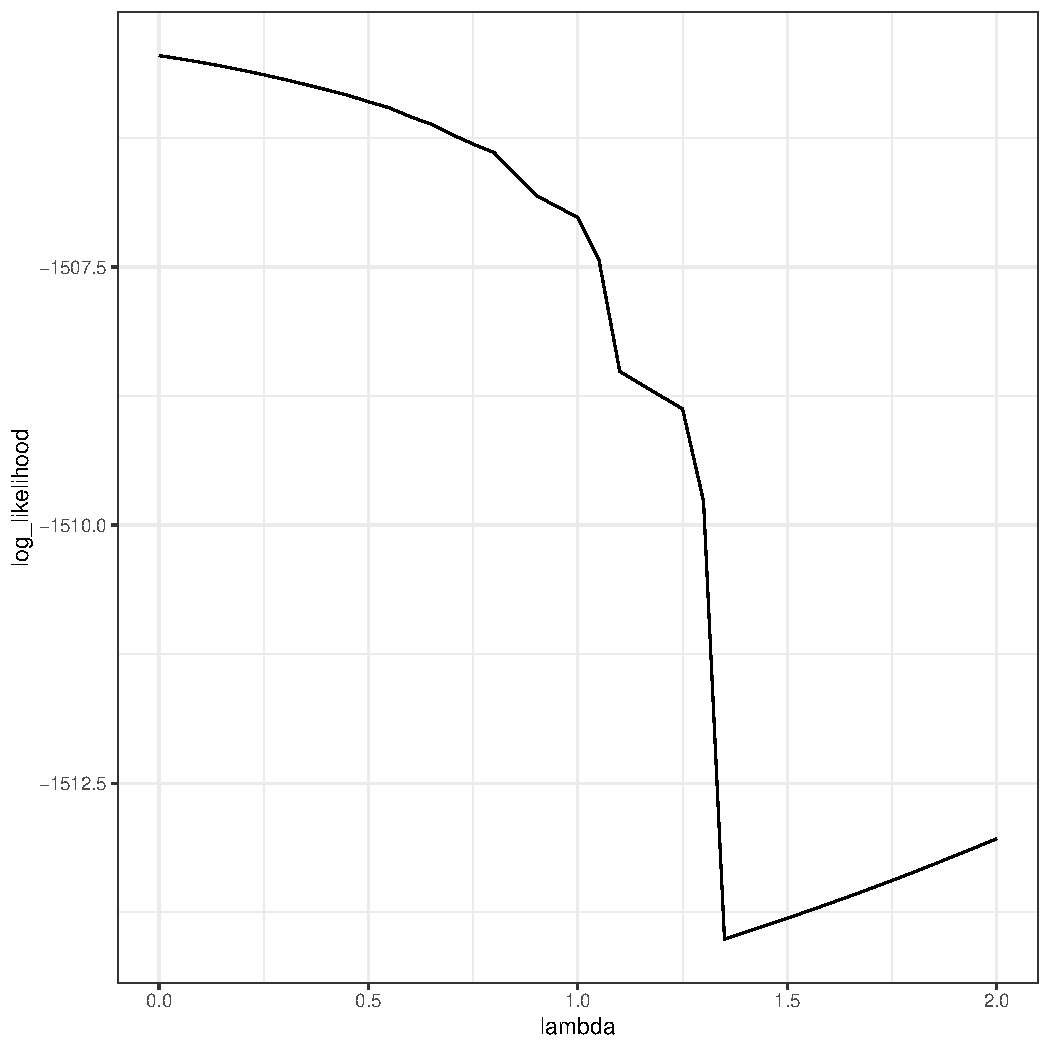
\includegraphics[width=\maxwidth]{figure/unnamed-chunk-5-1} 

\end{knitrout}


\end{frame}

\end{document}
